% Options for packages loaded elsewhere
\PassOptionsToPackage{unicode}{hyperref}
\PassOptionsToPackage{hyphens}{url}
%
\documentclass[
  8pt,
  ignorenonframetext,
]{beamer}
\title{Apprentissage supervisé - Régression}
\author{Mohamed Essaied Hamrita}
\date{IHEC - Sousse}

\usepackage{pgfpages}
\setbeamertemplate{caption}[numbered]
\setbeamertemplate{caption label separator}{: }
\setbeamercolor{caption name}{fg=normal text.fg}
\beamertemplatenavigationsymbolsempty
% Prevent slide breaks in the middle of a paragraph
\widowpenalties 1 10000
\raggedbottom
\setbeamertemplate{part page}{
  \centering
  \begin{beamercolorbox}[sep=16pt,center]{part title}
    \usebeamerfont{part title}\insertpart\par
  \end{beamercolorbox}
}
\setbeamertemplate{section page}{
  \centering
  \begin{beamercolorbox}[sep=12pt,center]{part title}
    \usebeamerfont{section title}\insertsection\par
  \end{beamercolorbox}
}
\setbeamertemplate{subsection page}{
  \centering
  \begin{beamercolorbox}[sep=8pt,center]{part title}
    \usebeamerfont{subsection title}\insertsubsection\par
  \end{beamercolorbox}
}
\AtBeginPart{
  \frame{\partpage}
}
\AtBeginSection{
  \ifbibliography
  \else
    \frame{\sectionpage}
  \fi
}
\AtBeginSubsection{
  \frame{\subsectionpage}
}
\usepackage{amsmath,amssymb}
\usepackage{lmodern}
\usepackage{iftex}
\ifPDFTeX
  \usepackage[T1]{fontenc}
  \usepackage[utf8]{inputenc}
  \usepackage{textcomp} % provide euro and other symbols
\else % if luatex or xetex
  \usepackage{unicode-math}
  \defaultfontfeatures{Scale=MatchLowercase}
  \defaultfontfeatures[\rmfamily]{Ligatures=TeX,Scale=1}
\fi
\usefonttheme{structurebold}
% Use upquote if available, for straight quotes in verbatim environments
\IfFileExists{upquote.sty}{\usepackage{upquote}}{}
\IfFileExists{microtype.sty}{% use microtype if available
  \usepackage[]{microtype}
  \UseMicrotypeSet[protrusion]{basicmath} % disable protrusion for tt fonts
}{}
\makeatletter
\@ifundefined{KOMAClassName}{% if non-KOMA class
  \IfFileExists{parskip.sty}{%
    \usepackage{parskip}
  }{% else
    \setlength{\parindent}{0pt}
    \setlength{\parskip}{6pt plus 2pt minus 1pt}}
}{% if KOMA class
  \KOMAoptions{parskip=half}}
\makeatother
\usepackage{xcolor}
\IfFileExists{xurl.sty}{\usepackage{xurl}}{} % add URL line breaks if available
\IfFileExists{bookmark.sty}{\usepackage{bookmark}}{\usepackage{hyperref}}
\hypersetup{
  pdftitle={Apprentissage supervisé - Régression},
  pdfauthor={Mohamed Essaied Hamrita},
  hidelinks,
  pdfcreator={LaTeX via pandoc}}
\urlstyle{same} % disable monospaced font for URLs
\newif\ifbibliography
\usepackage{color}
\usepackage{fancyvrb}
\newcommand{\VerbBar}{|}
\newcommand{\VERB}{\Verb[commandchars=\\\{\}]}
\DefineVerbatimEnvironment{Highlighting}{Verbatim}{commandchars=\\\{\}}
% Add ',fontsize=\small' for more characters per line
\usepackage{framed}
\definecolor{shadecolor}{RGB}{248,248,248}
\newenvironment{Shaded}{\begin{snugshade}}{\end{snugshade}}
\newcommand{\AlertTok}[1]{\textcolor[rgb]{0.94,0.16,0.16}{#1}}
\newcommand{\AnnotationTok}[1]{\textcolor[rgb]{0.56,0.35,0.01}{\textbf{\textit{#1}}}}
\newcommand{\AttributeTok}[1]{\textcolor[rgb]{0.77,0.63,0.00}{#1}}
\newcommand{\BaseNTok}[1]{\textcolor[rgb]{0.00,0.00,0.81}{#1}}
\newcommand{\BuiltInTok}[1]{#1}
\newcommand{\CharTok}[1]{\textcolor[rgb]{0.31,0.60,0.02}{#1}}
\newcommand{\CommentTok}[1]{\textcolor[rgb]{0.56,0.35,0.01}{\textit{#1}}}
\newcommand{\CommentVarTok}[1]{\textcolor[rgb]{0.56,0.35,0.01}{\textbf{\textit{#1}}}}
\newcommand{\ConstantTok}[1]{\textcolor[rgb]{0.00,0.00,0.00}{#1}}
\newcommand{\ControlFlowTok}[1]{\textcolor[rgb]{0.13,0.29,0.53}{\textbf{#1}}}
\newcommand{\DataTypeTok}[1]{\textcolor[rgb]{0.13,0.29,0.53}{#1}}
\newcommand{\DecValTok}[1]{\textcolor[rgb]{0.00,0.00,0.81}{#1}}
\newcommand{\DocumentationTok}[1]{\textcolor[rgb]{0.56,0.35,0.01}{\textbf{\textit{#1}}}}
\newcommand{\ErrorTok}[1]{\textcolor[rgb]{0.64,0.00,0.00}{\textbf{#1}}}
\newcommand{\ExtensionTok}[1]{#1}
\newcommand{\FloatTok}[1]{\textcolor[rgb]{0.00,0.00,0.81}{#1}}
\newcommand{\FunctionTok}[1]{\textcolor[rgb]{0.00,0.00,0.00}{#1}}
\newcommand{\ImportTok}[1]{#1}
\newcommand{\InformationTok}[1]{\textcolor[rgb]{0.56,0.35,0.01}{\textbf{\textit{#1}}}}
\newcommand{\KeywordTok}[1]{\textcolor[rgb]{0.13,0.29,0.53}{\textbf{#1}}}
\newcommand{\NormalTok}[1]{#1}
\newcommand{\OperatorTok}[1]{\textcolor[rgb]{0.81,0.36,0.00}{\textbf{#1}}}
\newcommand{\OtherTok}[1]{\textcolor[rgb]{0.56,0.35,0.01}{#1}}
\newcommand{\PreprocessorTok}[1]{\textcolor[rgb]{0.56,0.35,0.01}{\textit{#1}}}
\newcommand{\RegionMarkerTok}[1]{#1}
\newcommand{\SpecialCharTok}[1]{\textcolor[rgb]{0.00,0.00,0.00}{#1}}
\newcommand{\SpecialStringTok}[1]{\textcolor[rgb]{0.31,0.60,0.02}{#1}}
\newcommand{\StringTok}[1]{\textcolor[rgb]{0.31,0.60,0.02}{#1}}
\newcommand{\VariableTok}[1]{\textcolor[rgb]{0.00,0.00,0.00}{#1}}
\newcommand{\VerbatimStringTok}[1]{\textcolor[rgb]{0.31,0.60,0.02}{#1}}
\newcommand{\WarningTok}[1]{\textcolor[rgb]{0.56,0.35,0.01}{\textbf{\textit{#1}}}}
\setlength{\emergencystretch}{3em} % prevent overfull lines
\providecommand{\tightlist}{%
  \setlength{\itemsep}{0pt}\setlength{\parskip}{0pt}}
\setcounter{secnumdepth}{-\maxdimen} % remove section numbering
\setbeamertemplate{navigation symbols}{}
\setbeamertemplate{footline}[page number]
\ifLuaTeX
  \usepackage{selnolig}  % disable illegal ligatures
\fi

\begin{document}
\frame{\titlepage}

\begin{frame}[allowframebreaks]
  \tableofcontents[hideallsubsections]
\end{frame}
\begin{frame}
\definecolor{shadecolor}{RGB}{225, 225, 225}
\end{frame}

\hypertarget{introduction}{%
\section{Introduction}\label{introduction}}

\begin{frame}{Introduction}
L'apprentissage supervisé est classée dans deux catégories
d'algorithmes:\pause

\begin{itemize}
\tightlist
\item
  \(\color{red}{\bf{\text{Régression}:}}\) Un problème de régression se
  pose lorsque la variable étiquetée (labelled) est une valeur
  réelle.\pause 
\end{itemize}

Dans la littérature, il existe plusieurs types de modèles de régression
tels que la régression linéaire, la régression logistique, le SVM
(Support Vector Machine), NN (neural network) et KNN (K nearest
neighbour), \ldots \pause

\begin{itemize}
\tightlist
\item
  \(\color{red}{\bf{\text{Classification}:}}\) On parle d'un problème de
  classification lorsque la variable étiquetée est catégorielle (binaire
  ou multi-classes).\pause
\end{itemize}

Les modèles de classification comprennent la régression logistique,
l'arbre de décision (tree decision), la forêt aléatoire (random forest),
KNN et SVM.

\vspace*{3cm}
\end{frame}

\hypertarget{la-fonction-couxfbt-cost-loss-function}{%
\section{La fonction coût (Cost (loss)
function)}\label{la-fonction-couxfbt-cost-loss-function}}

\begin{frame}{La fonction coût (Cost (loss) function)}
L'apprentissage statistique supervisé repose sur une hypothèse qui
minimise le coût (la perte) moyen(ne) dans
l'\(\color{blue}{\bf{\text{échantillon}}}\). Ce qu'on appelle le
problème minimisation du coût.\pause

La fonction d'un prédicteur \(f\) est donné par:
\(\mathcal{R}(f)=\mathbb{E}\left(\ell\left(f(x)\right),y \right)\).

Le meilleur prédicteur est celui qui minimise cette fonction:
\(f^*=\min\left\{\mathcal{R}(f)\right\}\).\pause

L'estimateur de la fonction coût est: \[
\mathcal{R}_n(f)=\dfrac{1}{n}\sum_i\ell\left(f(x_i),y_i \right)
\]
\end{frame}

\hypertarget{la-ruxe9gression-linuxe9aire}{%
\section{La régression linéaire}\label{la-ruxe9gression-linuxe9aire}}

\begin{frame}{La régression linéaire}
La régression linéaire consiste à estimer \((k+1)\) paramètres dans une
relation \(\color{blue}{\bf linéaire}\) entre une variable dépendante
(target) et \(k\) variables indépendantes (features): \[
y_i=\beta_0 + \beta_1 x_{1i}+\ldots +\beta_k x_{ki}+\varepsilon_i\qquad \qquad (Y=X\beta +\varepsilon)
\]

\begin{itemize}
\item
  \(f\) est la relation linéaire entre \(y_i\) et \(x_{ki}\);
\item
  \(\ell\) peut être le coût de l'erreur quadratique: \[
  \ell(f(x),y)={\left(f(x)-y \right)}^2=\dfrac{1}{n}\sum_i {\left(x'_i\beta-y_i \right) }^2
  \]
\item
  Le meilleur prédicteur s'obtient en minimisant la fonction coût \[
  \widehat{f^*}=\min_{\beta}{\left(f(x)-y \right)}^2=\dfrac{1}{n}\sum_i {\left(x'_i\beta-y_i \right) }^2
  \]
\end{itemize}
\end{frame}

\begin{frame}[fragile]
\(\bf\color{blue}{\text{Implémentation sous R:}}\)

\begin{itemize}
\tightlist
\item
  Dataset and exploration: La bibliothèque \texttt{MASS} contient
  l'ensemble de données de \texttt{Boston}, qui enregistre la
  \texttt{medv} (valeur mediane des maisons) pour 506 quartiers de
  Boston. Nous chercherons à prédire \texttt{medv} à l'aide de 13
  prédicteurs tels que \texttt{rm} (nombre moyen de pièces par maison),
  \texttt{age} (âge moyen des maisons) et \texttt{lstat} (pourcentage de
  ménages à faible revenu).
\end{itemize}

\footnotesize

\begin{Shaded}
\begin{Highlighting}[]
\FunctionTok{library}\NormalTok{(MASS)  }
\FunctionTok{names}\NormalTok{(Boston)      }\CommentTok{\# Les noms des variables}
\end{Highlighting}
\end{Shaded}

\begin{verbatim}
 [1] "crim"    "zn"      "indus"   "chas"    "nox"     "rm"      "age"    
 [8] "dis"     "rad"     "tax"     "ptratio" "black"   "lstat"   "medv"   
\end{verbatim}

\begin{Shaded}
\begin{Highlighting}[]
\FunctionTok{any}\NormalTok{(}\FunctionTok{is.na}\NormalTok{(Boston)) }\CommentTok{\# y a t{-}il des valeurs manquantes?}
\end{Highlighting}
\end{Shaded}

\begin{verbatim}
[1] FALSE
\end{verbatim}

\normalsize
\end{frame}

\begin{frame}
\begin{itemize}
\tightlist
\item
  Model training and evaluation
\end{itemize}

Le problème fondamental de sur-estimation (overfitting) est que le
risque empirique, est biaisé à la baisse par rapport au risque de la
population. Nous pouvons éliminer ce biais de deux manières : (a) des
approches de ré-échantillonnage purement algorithmiques (train/test
(échantillonnage aléatoire simple (EAS)) et k-fold cross validation
(échantillonnage stratifié)) et (b) des estimateurs fondés sur la
théorie.\pause

\begin{center}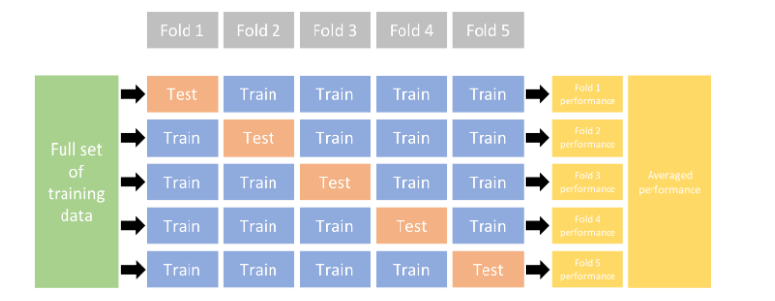
\includegraphics[width=0.7\linewidth,height=0.5\textheight]{fig/kcv} \end{center}
\end{frame}

\begin{frame}[fragile]
\begin{itemize}
\tightlist
\item
  Spit data
\end{itemize}

\footnotesize

\begin{Shaded}
\begin{Highlighting}[]
\FunctionTok{set.seed}\NormalTok{(}\DecValTok{0123}\NormalTok{); n}\OtherTok{=}\FunctionTok{nrow}\NormalTok{(Boston)}
\NormalTok{i\_train}\OtherTok{=}\FunctionTok{sample}\NormalTok{(}\DecValTok{1}\SpecialCharTok{:}\NormalTok{n, }\FunctionTok{round}\NormalTok{(}\FloatTok{0.7}\SpecialCharTok{*}\NormalTok{n))}
\NormalTok{train}\OtherTok{=}\NormalTok{Boston[i\_train,] ; test}\OtherTok{=}\NormalTok{Boston[}\SpecialCharTok{{-}}\NormalTok{i\_train,]}
\end{Highlighting}
\end{Shaded}

\normalsize

où encore, avec la bibliothèque \texttt{caret}

\footnotesize

\begin{Shaded}
\begin{Highlighting}[]
\FunctionTok{library}\NormalTok{(caret); }\FunctionTok{set.seed}\NormalTok{(}\DecValTok{0123}\NormalTok{)}
\NormalTok{i\_tr}\OtherTok{=}\FunctionTok{createDataPartition}\NormalTok{(Boston[,}\DecValTok{1}\NormalTok{], }\AttributeTok{p=}\FloatTok{0.7}\NormalTok{, }\AttributeTok{list=}\NormalTok{F)}
\NormalTok{train2}\OtherTok{=}\NormalTok{Boston[i\_tr,] ; test2}\OtherTok{=}\NormalTok{Boston[}\SpecialCharTok{{-}}\NormalTok{i\_tr,]}
\end{Highlighting}
\end{Shaded}

\normalsize
\end{frame}

\begin{frame}[fragile]
\begin{itemize}
\tightlist
\item
  Estimation
\end{itemize}

\footnotesize

\begin{Shaded}
\begin{Highlighting}[]
\NormalTok{mod1}\OtherTok{=}\FunctionTok{lm}\NormalTok{(medv }\SpecialCharTok{\textasciitilde{}}\NormalTok{ rm , }\AttributeTok{data=}\NormalTok{train); }\FunctionTok{summary}\NormalTok{(mod1)}
\end{Highlighting}
\end{Shaded}

\begin{verbatim}
Call:
lm(formula = medv ~ rm, data = train)

Residuals:
    Min      1Q  Median      3Q     Max 
-19.325  -2.586   0.028   2.829  39.073 

Coefficients:
            Estimate Std. Error t value Pr(>|t|)    
(Intercept) -32.6774     3.3137  -9.861   <2e-16 ***
rm            8.7735     0.5256  16.691   <2e-16 ***
---
Signif. codes:  0 '***' 0.001 '**' 0.01 '*' 0.05 '.' 0.1 ' ' 1

Residual standard error: 6.803 on 352 degrees of freedom
Multiple R-squared:  0.4418,    Adjusted R-squared:  0.4402 
F-statistic: 278.6 on 1 and 352 DF,  p-value: < 2.2e-16
\end{verbatim}

\normalsize
\end{frame}

\begin{frame}[fragile]
\footnotesize

\begin{Shaded}
\begin{Highlighting}[]
\NormalTok{mod2}\OtherTok{=}\FunctionTok{update}\NormalTok{(mod1, .}\SpecialCharTok{\textasciitilde{}}\NormalTok{. }\SpecialCharTok{+}\NormalTok{ lstat , }\AttributeTok{data=}\NormalTok{train)}
\FunctionTok{summary}\NormalTok{(mod2)}
\end{Highlighting}
\end{Shaded}

\begin{verbatim}
Call:
lm(formula = medv ~ rm + lstat, data = train)

Residuals:
    Min      1Q  Median      3Q     Max 
-12.468  -3.470  -1.154   1.753  27.410 

Coefficients:
            Estimate Std. Error t value Pr(>|t|)    
(Intercept)  1.98609    3.82193    0.52    0.604    
rm           4.58297    0.54042    8.48 6.33e-16 ***
lstat       -0.66666    0.05145  -12.96  < 2e-16 ***
---
Signif. codes:  0 '***' 0.001 '**' 0.01 '*' 0.05 '.' 0.1 ' ' 1

Residual standard error: 5.603 on 351 degrees of freedom
Multiple R-squared:  0.6224,    Adjusted R-squared:  0.6202 
F-statistic: 289.3 on 2 and 351 DF,  p-value: < 2.2e-16
\end{verbatim}

\normalsize
\end{frame}

\begin{frame}[fragile]
\footnotesize

\begin{Shaded}
\begin{Highlighting}[]
\NormalTok{mod3}\OtherTok{=}\FunctionTok{update}\NormalTok{(mod2, .}\SpecialCharTok{\textasciitilde{}}\NormalTok{. }\SpecialCharTok{+}\NormalTok{ age, }\AttributeTok{data=}\NormalTok{train)}
\FunctionTok{summary}\NormalTok{(mod3)}
\end{Highlighting}
\end{Shaded}

\begin{verbatim}
Call:
lm(formula = medv ~ rm + lstat + age, data = train)

Residuals:
    Min      1Q  Median      3Q     Max 
-12.928  -3.442  -1.175   1.915  26.430 

Coefficients:
            Estimate Std. Error t value Pr(>|t|)    
(Intercept)  1.96544    3.81823   0.515    0.607    
rm           4.49245    0.54437   8.253  3.2e-15 ***
lstat       -0.71310    0.06261 -11.389  < 2e-16 ***
age          0.01723    0.01327   1.299    0.195    
---
Signif. codes:  0 '***' 0.001 '**' 0.01 '*' 0.05 '.' 0.1 ' ' 1

Residual standard error: 5.598 on 350 degrees of freedom
Multiple R-squared:  0.6242,    Adjusted R-squared:  0.621 
F-statistic: 193.8 on 3 and 350 DF,  p-value: < 2.2e-16
\end{verbatim}

\normalsize
\end{frame}

\begin{frame}[fragile]
On a estimé 3 modèles. La question qui se pose: quel est le meilleur
modèle ? \pause

Pour répondre à cette question, on doit définir ce que veut dire
``meilleur''. Dans ce cas, on utilisera RMSE comme métrique et la
validation croisée comme approche de re-échantillonnage.

\footnotesize

\begin{Shaded}
\begin{Highlighting}[]
\FunctionTok{set.seed}\NormalTok{(}\DecValTok{123}\NormalTok{)  }
\NormalTok{(cv\_mod1 }\OtherTok{\textless{}{-}} \FunctionTok{train}\NormalTok{(}\AttributeTok{form =}\NormalTok{ medv }\SpecialCharTok{\textasciitilde{}}\NormalTok{ rm, }
  \AttributeTok{data =}\NormalTok{ train, }\AttributeTok{method =} \StringTok{"lm"}\NormalTok{,}
  \AttributeTok{trControl =} \FunctionTok{trainControl}\NormalTok{(}\AttributeTok{method =} \StringTok{"cv"}\NormalTok{, }\AttributeTok{number =} \DecValTok{10}\NormalTok{)))}
\end{Highlighting}
\end{Shaded}

\begin{verbatim}
Linear Regression 

354 samples
  1 predictor

No pre-processing
Resampling: Cross-Validated (10 fold) 
Summary of sample sizes: 318, 319, 318, 319, 319, 319, ... 
Resampling results:

  RMSE      Rsquared   MAE     
  6.568065  0.4999459  4.517952

Tuning parameter 'intercept' was held constant at a value of TRUE
\end{verbatim}

\normalsize
\end{frame}

\begin{frame}[fragile]
\footnotesize

\begin{Shaded}
\begin{Highlighting}[]
\FunctionTok{set.seed}\NormalTok{(}\DecValTok{123}\NormalTok{)  }
\NormalTok{(cv\_mod2 }\OtherTok{\textless{}{-}} \FunctionTok{train}\NormalTok{(}\AttributeTok{form =}\NormalTok{ medv }\SpecialCharTok{\textasciitilde{}}\NormalTok{ rm }\SpecialCharTok{+}\NormalTok{ lstat, }
  \AttributeTok{data =}\NormalTok{ train, }\AttributeTok{method =} \StringTok{"lm"}\NormalTok{,}
  \AttributeTok{trControl =} \FunctionTok{trainControl}\NormalTok{(}\AttributeTok{method =} \StringTok{"cv"}\NormalTok{, }\AttributeTok{number =} \DecValTok{10}\NormalTok{)))}
\end{Highlighting}
\end{Shaded}

\begin{verbatim}
Linear Regression 

354 samples
  2 predictor

No pre-processing
Resampling: Cross-Validated (10 fold) 
Summary of sample sizes: 318, 319, 318, 319, 319, 319, ... 
Resampling results:

  RMSE     Rsquared   MAE   
  5.50875  0.6357689  4.0166

Tuning parameter 'intercept' was held constant at a value of TRUE
\end{verbatim}

\normalsize
\end{frame}

\begin{frame}[fragile]
\footnotesize

\begin{Shaded}
\begin{Highlighting}[]
\FunctionTok{set.seed}\NormalTok{(}\DecValTok{123}\NormalTok{)  }
\NormalTok{(cv\_mod3 }\OtherTok{\textless{}{-}} \FunctionTok{train}\NormalTok{(}\AttributeTok{form =}\NormalTok{ medv }\SpecialCharTok{\textasciitilde{}}\NormalTok{ rm }\SpecialCharTok{+}\NormalTok{ lstat }\SpecialCharTok{+}\NormalTok{ age, }
  \AttributeTok{data =}\NormalTok{ train, }\AttributeTok{method =} \StringTok{"lm"}\NormalTok{,}
  \AttributeTok{trControl =} \FunctionTok{trainControl}\NormalTok{(}\AttributeTok{method =} \StringTok{"cv"}\NormalTok{, }\AttributeTok{number =} \DecValTok{10}\NormalTok{)))}
\end{Highlighting}
\end{Shaded}

\begin{verbatim}
Linear Regression 

354 samples
  3 predictor

No pre-processing
Resampling: Cross-Validated (10 fold) 
Summary of sample sizes: 318, 319, 318, 319, 319, 319, ... 
Resampling results:

  RMSE      Rsquared   MAE     
  5.577216  0.6290893  4.048824

Tuning parameter 'intercept' was held constant at a value of TRUE
\end{verbatim}

\normalsize
\end{frame}

\begin{frame}[fragile]
\footnotesize

\begin{Shaded}
\begin{Highlighting}[]
\CommentTok{\# Extract out of sample performance measures}
\FunctionTok{summary}\NormalTok{(}\FunctionTok{resamples}\NormalTok{(}\FunctionTok{list}\NormalTok{(}\AttributeTok{model1 =}\NormalTok{ cv\_mod1, }\AttributeTok{model2 =}\NormalTok{ cv\_mod2,}
                       \AttributeTok{model3 =}\NormalTok{ cv\_mod3)))}
\end{Highlighting}
\end{Shaded}

\begin{verbatim}
Call:
summary.resamples(object = resamples(list(model1 = cv_mod1, model2 =
 cv_mod2, model3 = cv_mod3)))

Models: model1, model2, model3 
Number of resamples: 10 

MAE 
           Min.  1st Qu.   Median     Mean  3rd Qu.     Max. NA's
model1 3.679413 3.789617 4.171966 4.517952 4.755100 7.561154    0
model2 2.666590 3.587005 3.803046 4.016600 4.392750 6.279433    0
model3 2.810045 3.649151 3.806138 4.048824 4.410426 6.322432    0

RMSE 
           Min.  1st Qu.   Median     Mean  3rd Qu.      Max. NA's
model1 4.994818 5.231666 6.008484 6.568065 7.007573 12.070129    0
model2 3.132182 4.933731 5.178013 5.508750 6.024353  9.429550    0
model3 3.311719 4.892822 5.251309 5.577216 6.236043  9.544912    0

Rsquared 
             Min.   1st Qu.    Median      Mean   3rd Qu.      Max. NA's
model1 0.04276741 0.3401524 0.5536225 0.4999459 0.6888395 0.7678734    0
model2 0.32808065 0.5486184 0.6440678 0.6357689 0.7665443 0.8070292    0
model3 0.31286706 0.5440675 0.6521460 0.6290893 0.7546747 0.7883733    0
\end{verbatim}

\normalsize
\end{frame}

\begin{frame}[fragile]
L'estimation du modèle linéaire se repose sur le respect de quelques
hypothèses (linéarité, variance constante, erreurs non corrolées,
\ldots)\pause

Donc, l'étape de la validation consiste à vérifier si ces hypothèses
sont bien remplies à travers des graphiques et des tests statistiques.
\vspace*{1cm}

\footnotesize

\begin{Shaded}
\begin{Highlighting}[]
\NormalTok{p1}\OtherTok{=}\FunctionTok{ggplot}\NormalTok{(train,}\FunctionTok{aes}\NormalTok{(medv, rm))}\SpecialCharTok{+}\FunctionTok{geom\_point}\NormalTok{(}\AttributeTok{size=}\DecValTok{1}\NormalTok{, }\AttributeTok{alpha=}\FloatTok{0.4}\NormalTok{)}\SpecialCharTok{+}\FunctionTok{geom\_smooth}\NormalTok{(}\AttributeTok{se=}\NormalTok{F)}

\NormalTok{p2}\OtherTok{=}\FunctionTok{ggplot}\NormalTok{(train,}\FunctionTok{aes}\NormalTok{(medv, rm))}\SpecialCharTok{+}\FunctionTok{geom\_point}\NormalTok{(}\AttributeTok{size=}\DecValTok{1}\NormalTok{, }\AttributeTok{alpha=}\FloatTok{0.4}\NormalTok{)}\SpecialCharTok{+}\FunctionTok{geom\_smooth}\NormalTok{(}\AttributeTok{method=}\StringTok{"lm"}\NormalTok{,}\AttributeTok{se=}\NormalTok{F)}\SpecialCharTok{+}
  \FunctionTok{scale\_y\_log10}\NormalTok{(}\StringTok{"rm"}\NormalTok{)}
\end{Highlighting}
\end{Shaded}

\normalsize \vspace*{2cm}
\end{frame}

\begin{frame}[fragile]
\footnotesize

\begin{Shaded}
\begin{Highlighting}[]
\NormalTok{gridExtra}\SpecialCharTok{::}\FunctionTok{grid.arrange}\NormalTok{(p1,p2, }\AttributeTok{nrow=}\DecValTok{1}\NormalTok{)}
\end{Highlighting}
\end{Shaded}

\begin{center}\includegraphics[width=1\linewidth,height=0.65\textheight]{chap2_files/figure-beamer/unnamed-chunk-13-1} \end{center}

\normalsize
\end{frame}

\begin{frame}[fragile]
L'homoscédasticité: \vspace*{0.25cm}

\footnotesize

\begin{Shaded}
\begin{Highlighting}[]
\NormalTok{p11}\OtherTok{=}\FunctionTok{ggplot}\NormalTok{(cv\_mod1}\SpecialCharTok{$}\NormalTok{finalModel, }\FunctionTok{aes}\NormalTok{(}\AttributeTok{x =}\NormalTok{ .fitted, }\AttributeTok{y =}\NormalTok{ .resid))}\SpecialCharTok{+} \FunctionTok{geom\_point}\NormalTok{()}\SpecialCharTok{+} 
  \FunctionTok{geom\_hline}\NormalTok{(}\AttributeTok{yintercept =} \DecValTok{0}\NormalTok{) }\SpecialCharTok{+}  \FunctionTok{labs}\NormalTok{(}\AttributeTok{title=}\StringTok{\textquotesingle{}Residual vs. Fitted Values Plot\textquotesingle{}}\NormalTok{, }\AttributeTok{x=}\StringTok{\textquotesingle{}Fitted Values\textquotesingle{}}\NormalTok{, }
                                     \AttributeTok{y=}\StringTok{\textquotesingle{}Residuals\textquotesingle{}}\NormalTok{)}

\NormalTok{p12}\OtherTok{=}\FunctionTok{ggplot}\NormalTok{(cv\_mod2}\SpecialCharTok{$}\NormalTok{finalModel, }\FunctionTok{aes}\NormalTok{(}\AttributeTok{x =}\NormalTok{ .fitted, }\AttributeTok{y =}\NormalTok{ .resid)) }\SpecialCharTok{+}  \FunctionTok{geom\_point}\NormalTok{() }\SpecialCharTok{+}
 \FunctionTok{geom\_hline}\NormalTok{(}\AttributeTok{yintercept =} \DecValTok{0}\NormalTok{) }\SpecialCharTok{+}   \FunctionTok{labs}\NormalTok{(}\AttributeTok{title=}\StringTok{\textquotesingle{}Residual vs. Fitted Values Plot\textquotesingle{}}\NormalTok{, }\AttributeTok{x=}\StringTok{\textquotesingle{}Fitted Values\textquotesingle{}}\NormalTok{, }
                                     \AttributeTok{y=}\StringTok{\textquotesingle{}Residuals\textquotesingle{}}\NormalTok{)}

\NormalTok{p13}\OtherTok{=}\FunctionTok{ggplot}\NormalTok{(cv\_mod3}\SpecialCharTok{$}\NormalTok{finalModel, }\FunctionTok{aes}\NormalTok{(}\AttributeTok{x =}\NormalTok{ .fitted, }\AttributeTok{y =}\NormalTok{ .resid)) }\SpecialCharTok{+}\FunctionTok{geom\_point}\NormalTok{() }\SpecialCharTok{+} 
  \FunctionTok{geom\_hline}\NormalTok{(}\AttributeTok{yintercept =} \DecValTok{0}\NormalTok{) }\SpecialCharTok{+}  \FunctionTok{labs}\NormalTok{(}\AttributeTok{title=}\StringTok{\textquotesingle{}Residual vs. Fitted Values Plot\textquotesingle{}}\NormalTok{, }\AttributeTok{x=}\StringTok{\textquotesingle{}Fitted Values\textquotesingle{}}\NormalTok{, }
                                     \AttributeTok{y=}\StringTok{\textquotesingle{}Residuals\textquotesingle{}}\NormalTok{)}

\NormalTok{gridExtra}\SpecialCharTok{::}\FunctionTok{grid.arrange}\NormalTok{(p11,p12,p13,}\AttributeTok{nrow=}\DecValTok{1}\NormalTok{)}
\end{Highlighting}
\end{Shaded}

\begin{center}\includegraphics[width=1\linewidth,height=0.4\textheight]{chap2_files/figure-beamer/unnamed-chunk-14-1} \end{center}

\normalsize
\end{frame}

\begin{frame}[fragile]
L'autocorrelation: pour tester graphiquement si les erreurs sont
indépendantes, on peut faire recours à la fonction
\texttt{checkresiduals()}de la bibliothèque \texttt{forecast}.
\vspace*{0.25cm}

\begin{Shaded}
\begin{Highlighting}[]
\NormalTok{forecast}\SpecialCharTok{::}\FunctionTok{checkresiduals}\NormalTok{(cv\_mod1)}
\end{Highlighting}
\end{Shaded}

\begin{center}\includegraphics[height=0.8\textheight]{chap2_files/figure-beamer/unnamed-chunk-15-1} \end{center}
\end{frame}

\begin{frame}[fragile]
Une fois, le modèle est validé, on passe à tester la précision des
prévisions du modèle. Ceci se fait en déterminant la prévision sur la
partie \texttt{test} et la comparer par la vrai valeur.

\begin{Shaded}
\begin{Highlighting}[]
\NormalTok{pred}\OtherTok{=}\FunctionTok{predict}\NormalTok{(cv\_mod1, }\AttributeTok{newdata =}\NormalTok{ test)}
\NormalTok{rmse}\OtherTok{=}\FunctionTok{sqrt}\NormalTok{(}\FunctionTok{mean}\NormalTok{((test}\SpecialCharTok{$}\NormalTok{medv}\SpecialCharTok{{-}}\NormalTok{pred)}\SpecialCharTok{\^{}}\DecValTok{2}\NormalTok{)); rmse}
\end{Highlighting}
\end{Shaded}

\begin{verbatim}
[1] 6.177801
\end{verbatim}

\begin{Shaded}
\begin{Highlighting}[]
\NormalTok{rmae}\OtherTok{=}\FunctionTok{sqrt}\NormalTok{(}\FunctionTok{mean}\NormalTok{(}\FunctionTok{abs}\NormalTok{(test}\SpecialCharTok{$}\NormalTok{medv}\SpecialCharTok{{-}}\NormalTok{pred))); rmae}
\end{Highlighting}
\end{Shaded}

\begin{verbatim}
[1] 2.103623
\end{verbatim}
\end{frame}

\begin{frame}[fragile]
\footnotesize

\begin{Shaded}
\begin{Highlighting}[]
\NormalTok{dd}\OtherTok{=}\FunctionTok{data.frame}\NormalTok{(}\AttributeTok{TrueVal=}\NormalTok{test}\SpecialCharTok{$}\NormalTok{medv,}\AttributeTok{PredVal=}\NormalTok{pred)}
\NormalTok{p3}\OtherTok{=}\FunctionTok{ggplot}\NormalTok{(dd, }\FunctionTok{aes}\NormalTok{(}\AttributeTok{x=}\DecValTok{1}\SpecialCharTok{:}\FunctionTok{nrow}\NormalTok{(dd)))}\SpecialCharTok{+}
  \FunctionTok{geom\_line}\NormalTok{(}\FunctionTok{aes}\NormalTok{(}\AttributeTok{y=}\NormalTok{TrueVal))}\SpecialCharTok{+}
  \FunctionTok{geom\_line}\NormalTok{(}\FunctionTok{aes}\NormalTok{(}\AttributeTok{y=}\NormalTok{PredVal), }\AttributeTok{color=}\StringTok{"darkred"}\NormalTok{)}\SpecialCharTok{+}
  \FunctionTok{labs}\NormalTok{(}\AttributeTok{x=}\StringTok{""}\NormalTok{, }\AttributeTok{y=}\StringTok{""}\NormalTok{)}
\NormalTok{p3}
\end{Highlighting}
\end{Shaded}

\begin{center}\includegraphics[width=0.9\linewidth,height=0.7\textheight]{chap2_files/figure-beamer/unnamed-chunk-17-1} \end{center}

\normalsize
\end{frame}

\end{document}
